\documentclass[conference]{IEEEtran}
\IEEEoverridecommandlockouts
\raggedbottom

\usepackage{cite}
\usepackage{amsmath,amssymb,amsfonts}
\usepackage{algorithmic}
\usepackage{graphicx}
\usepackage{textcomp}
\usepackage{xcolor}
\usepackage{float}
\usepackage{url}
\usepackage[utf8]{inputenc}
\usepackage[T1]{fontenc}
\usepackage[spanish]{babel}

\addto\captionsspanish{
  \renewcommand{\abstractname}{Abstract}
  \renewcommand{\IEEEkeywordsname}{Keywords}
}
\renewcommand{\abstractname}{Abstract}
\renewcommand{\IEEEkeywordsname}{Keywords}
\def\BibTeX{{\rm B\kern-.05em{\sc i\kern-.025em b}\kern-.08em
    T\kern-.1667em\lower.7ex\hbox{E}\kern-.125emX}}

\begin{document}

\title{Práctica 3: De radiofrecuencia a la envolvente compleja\\
{\footnotesize \textsuperscript{*} \url{https://github.com/edwinfarid31/2026_1_CommII_A1_G1/tree/Practica_3/PRACTICA_3/INFORME}}
\thanks{COMUNICACIONES II: 2026-1-27145-A1}
}

\author{
\IEEEauthorblockN{Edwin Farid Bolaño Perez}\
{\small Código: 2212264}
\IEEEauthorblockA{\textit{Universidad Industrial de Santander} \\
Bucaramanga, Colombia \\
edwin2212264@correo.uis.edu.co}
\and
\IEEEauthorblockN{Sergio Andrés Cárdenas}\
{\small Código: 2222243}
\IEEEauthorblockA{\textit{Universidad Industrial de Santander} \\
Bucaramanga, Colombia \\
sergio2222243@correo.uis.edu.co
}
\and
\IEEEauthorblockN{Johan Sebastian Fandino Ruiz}\
{\small Código: 2204271}
\IEEEauthorblockA{\textit{Universidad Industrial de Santander} \\
Bucaramanga, Colombia \\
Johan2204271@correo.uis.edu.co}
}

\maketitle

\begin{abstract}
This report analyzes the conversion of Radio Frequency (RF) signals to Complex Envelope (CE) for OOK, BPSK, and FSK modulations. The study focuses on the structural configuration of in-phase and quadrature components, evaluating the impact of interpolation filters and frequency deviation limits. Results demonstrate that CE representation optimizes baseband processing while maintaining signal integrity, provided that Nyquist sampling criteria and symbol-per-symbol constraints are satisfied.
\end{abstract}

\begin{IEEEkeywords}
BPSK, complex envelope, digital modulation, FSK, frequency deviation, GNU Radio, Nyquist criteria, RF conversion, samples per symbol (SPS).
\end{IEEEkeywords}

\section{Introducción}
La representación en Envolvente Compleja (EC) es una técnica esencial en telecomunicaciones que simplifica el procesamiento de señales de Radiofrecuencia (RF). Al trasladar la información a banda base, se facilita el análisis de fase y amplitud sin la carga computacional de la portadora de alta frecuencia. En este informe se evalúa la implementación de modulaciones digitales y se determinan los límites técnicos de muestreo y desviación de frecuencia necesarios para una reconstrucción fiel de la señal.

\section{Metodología y resultados}
Se diseñó un sistema de procesamiento donde las señales de información se integran mediante componentes en fase ($I$) y cuadratura ($Q$). Se estableció que para esquemas de fase como BPSK se utiliza la rama superior del sistema, mientras que para variaciones de frecuencia como FSK se emplea la rama de cuadratura. Se analizó la ubicación del bloque de interpolación, determinando que su posición es crítica antes de la mezcla para evitar distorsiones en la fase instantánea. Las condiciones de operación se fundamentan en el criterio de Nyquist [1].

\subsection{Modulación On-Ooff Keying (OOK)}
La modulación por desplazamiento de amplitud (OOK, On-Off Keying) se define como una técnica de transmisión digital fundamentada en la conmutación de la amplitud de una señal portadora para la representación de datos binarios. Como variante simplificada del esquema ASK (Amplitude Shift Keying), el proceso consiste en habilitar o inhabilitar la presencia de la portadora en función del bit transmitido. Tal como se ilustra en la Fig. 1, este comportamiento genera una señal discontinua donde la ausencia de energía se asocia unívocamente a un estado lógico, permitiendo una identificación directa de los símbolos en el dominio del tiempo.


\begin{figure}[H]
    \centering
    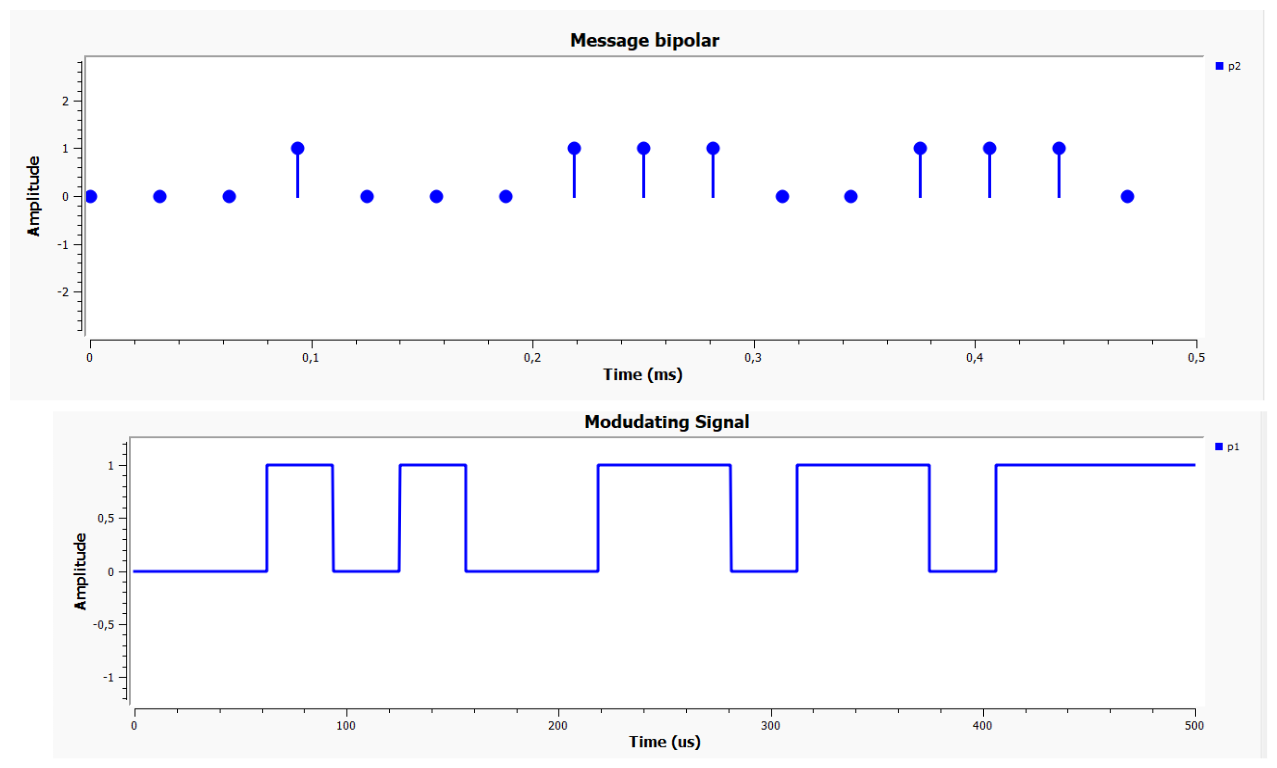
\includegraphics[width=0.85\columnwidth]{images/mensaje.png}
    \caption{mensaje}
    \label{fig:mensaje}
\end{figure}

En este esquema de modulación, la representación de cada bit se ejecuta bajo los siguientes criterios:

\begin{itemize}
    \item El bit 1 se transmite empleando una señal portadora con amplitud $A$.
    \item El bit 0 se define mediante la ausencia total de señal (amplitud nula).
\end{itemize}

Matemáticamente, la señal se expresa mediante la siguiente función por partes:

\begin{equation}
    s(t) =
    \begin{cases}
        A \cos(2\pi f_c t), & \text{si el bit es 1} \\
        0, & \text{si el bit es 0}
    \end{cases}
\end{equation}

Se determinó que la modulación OOK destaca por su sencillez en la implementación y su eficiencia energética, debido a que se evita la transmisión de potencia durante los estados lógicos '0'. No obstante, se analizó que este sistema presenta una mayor sensibilidad ante el ruido en comparación con técnicas que codifican la información en fase o frecuencia. Asimismo, se estableció que la robustez del sistema se encuentra supeditada a la frecuencia de la portadora (\textit{carrier}) seleccionada para la implementación.


\begin{figure}[H]
    \centering
    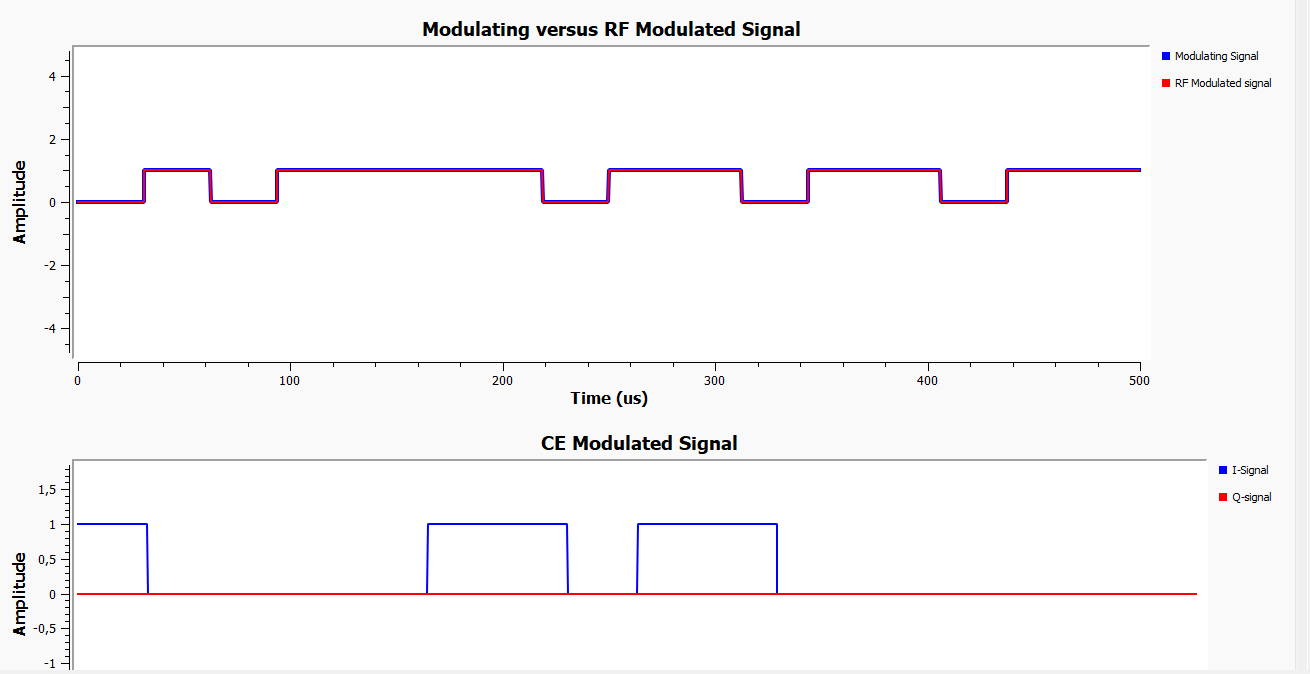
\includegraphics[width=0.9\columnwidth]{images/ook-rf-modulated-time-domain-fc-0.png}
    \caption{OOK RF Modulated/Time Domain Fc=0}
    \label{fig:ook_rf_modulated_time_domain_fc_0}
\end{figure}


\begin{figure}[H]
    \centering
    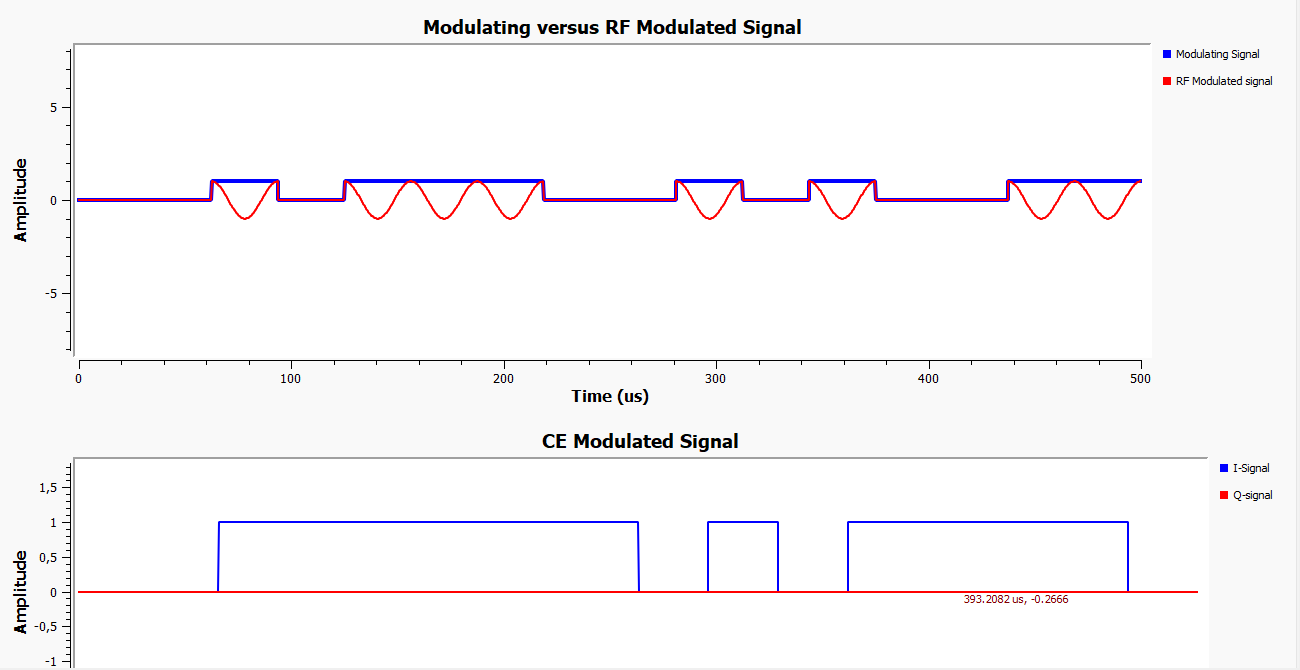
\includegraphics[width=0.9\columnwidth]{images/ook-rf-modulated-time-domain-fc-32k.png}
    \caption{OOK RF Modulated/Time Domain Fc=32k}
    \label{fig:ook_rf_modulated_time_domain_fc_32k}
\end{figure}


\begin{figure}[H]
    \centering
    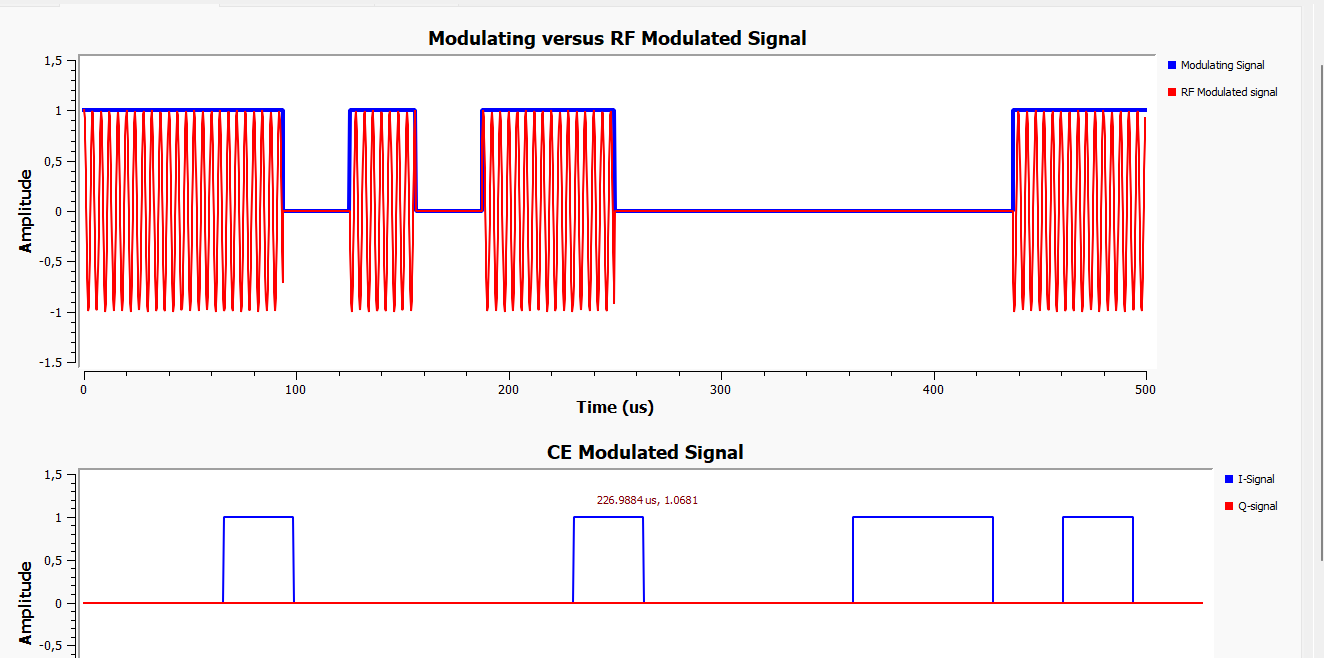
\includegraphics[width=0.9\columnwidth]{images/ook-rf-modulated-time-domain-fc-250k.png}
    \caption{OOK RF Modulated/Time Domain Fc=250k}
    \label{fig:ook_rf_modulated_time_domain_fc_250k}
\end{figure}
Este esquema de modulación se emplea en aplicaciones de bajo consumo y corto alcance, tales como controles remotos por infrarrojo, sistemas de comunicación óptica y diversos transmisores de radiofrecuencia digitales. Por otra parte, se ejecuta el análisis del comportamiento de la modulación en el dominio de la frecuencia.


\begin{figure}[H]
    \centering
    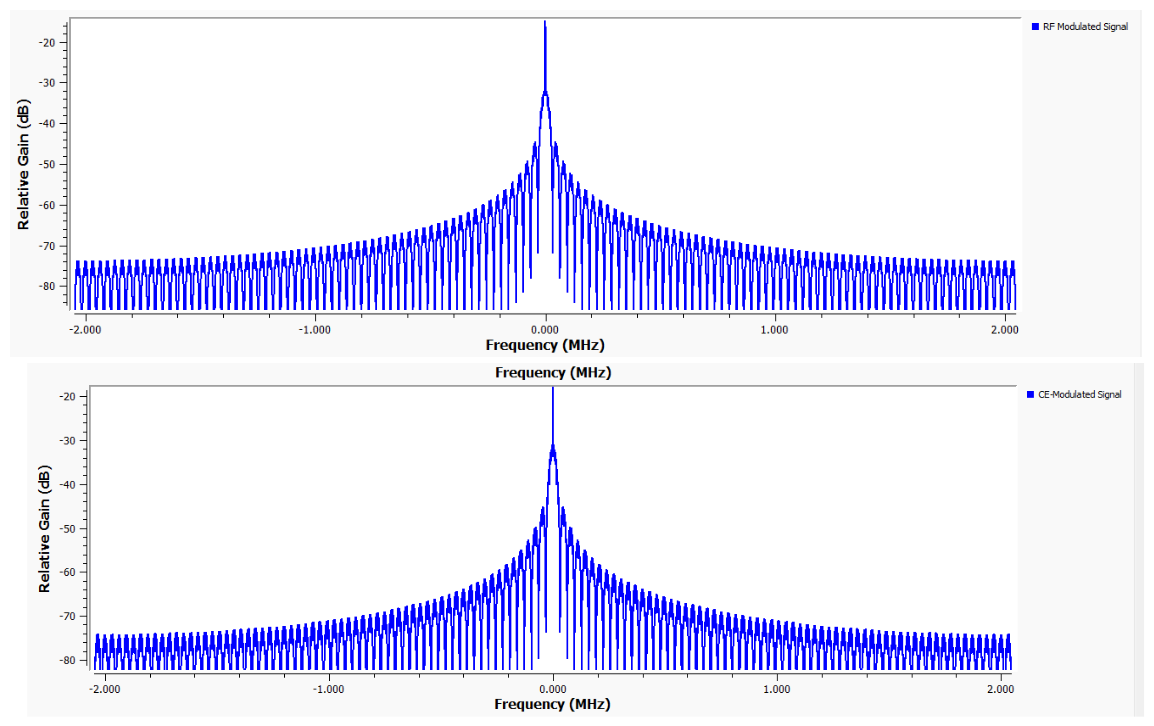
\includegraphics[width=0.9\columnwidth]{images/ook-rf-modulated-freq-domain-fc-0.png}
    \caption{OOK RF Modulated/Freq Domain Fc=0}
    \label{fig:ook_rf_modulated_freq_domain_fc_0}
\end{figure}



\begin{figure}[H]
    \centering
    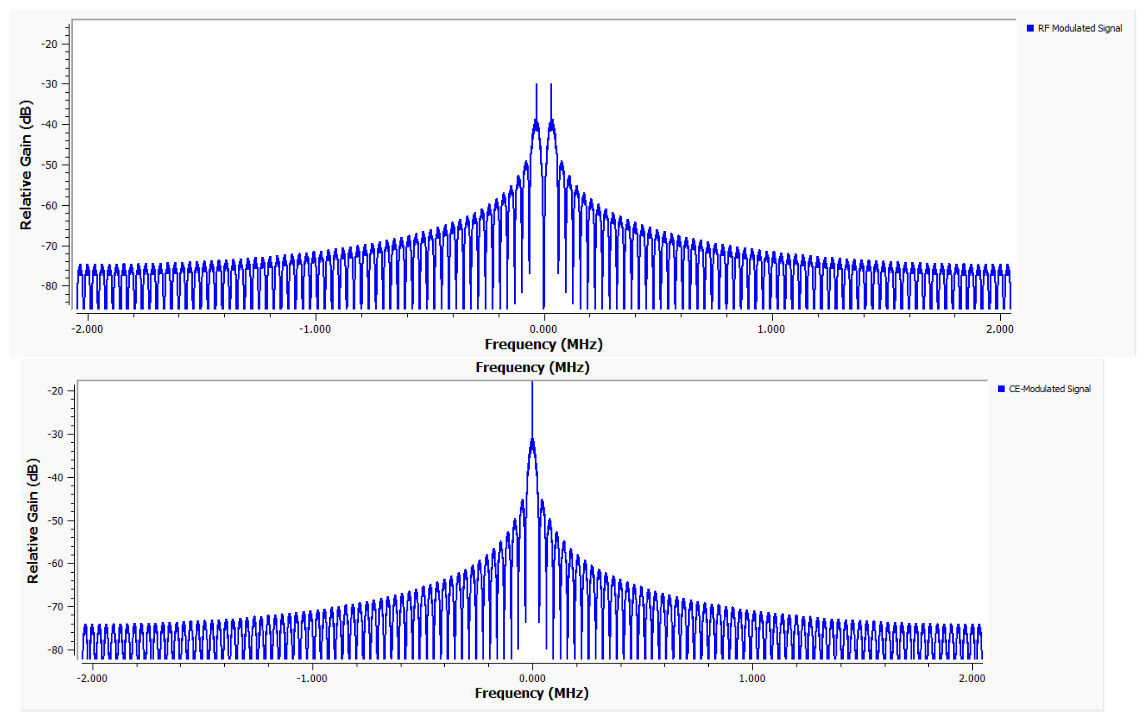
\includegraphics[width=0.9\columnwidth]{images/ook-rf-modulated-freq-domain-fc-32k.png}
    \caption{OOK RF Modulated/Freq Domain Fc=32k}
    \label{fig:ook_rf_modulated_freq_domain_fc_32k}
\end{figure}


\begin{figure}[H]
    \centering
    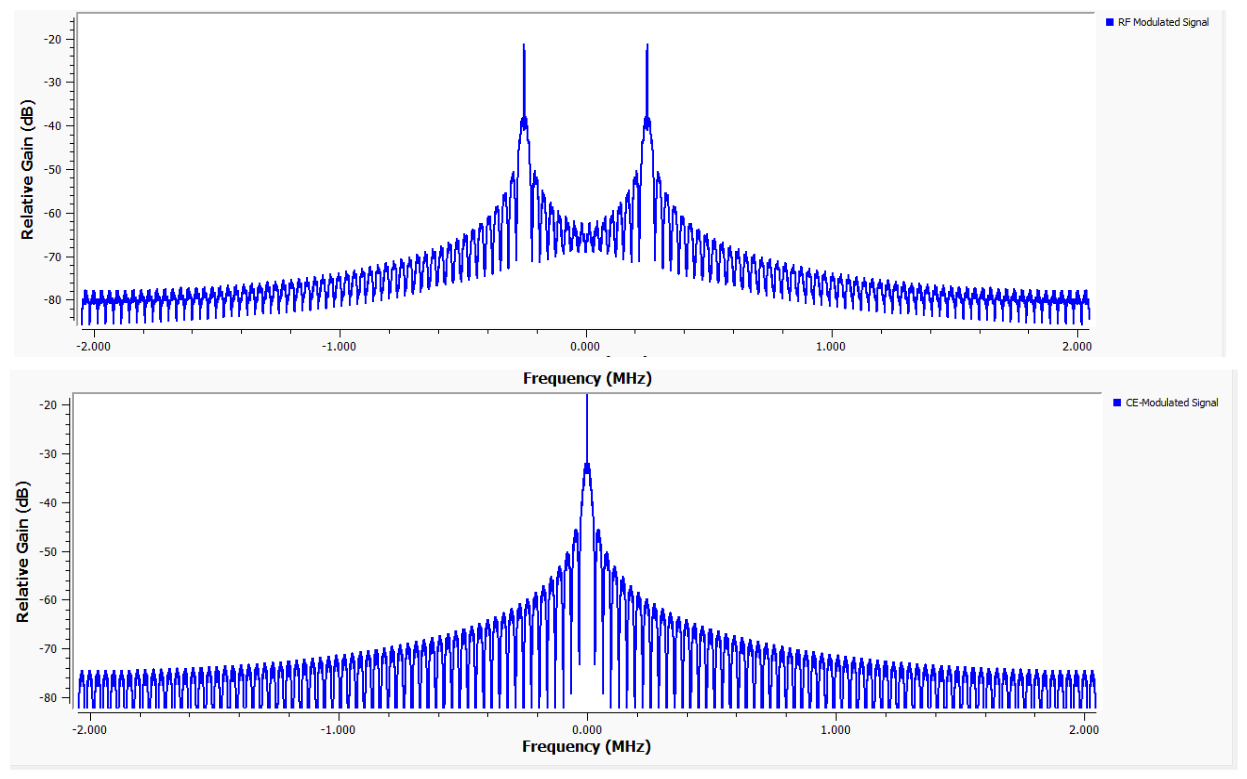
\includegraphics[width=0.9\columnwidth]{images/ook-rf-modulated-freq-domain-fc-250k.png}
    \caption{OOK RF Modulated/Freq Domain Fc=250k}
    \label{fig:ook_rf_modulated_freq_domain_fc_250k}
\end{figure}

\begin{itemize}
\item \textbf{Lóbulo principal (Fig. 5):} Se ubica centrado en la frecuencia portadora $f_c$ con amplitud máxima.
\item \textbf{Ancho de banda en la figura 7:} Se estima como $BW \approx \frac{R_b}{SPS} = \frac{32k}{4} = 8 \text{ kHz}$ por lóbulo.
\item \textbf{Lóbulos laterales (Fig. 8):} Se encuentran distribuidos simétricamente en torno a $f_c$, con decaimiento progresivo.
\end{itemize}

\begin{figure}[H]
    \centering
    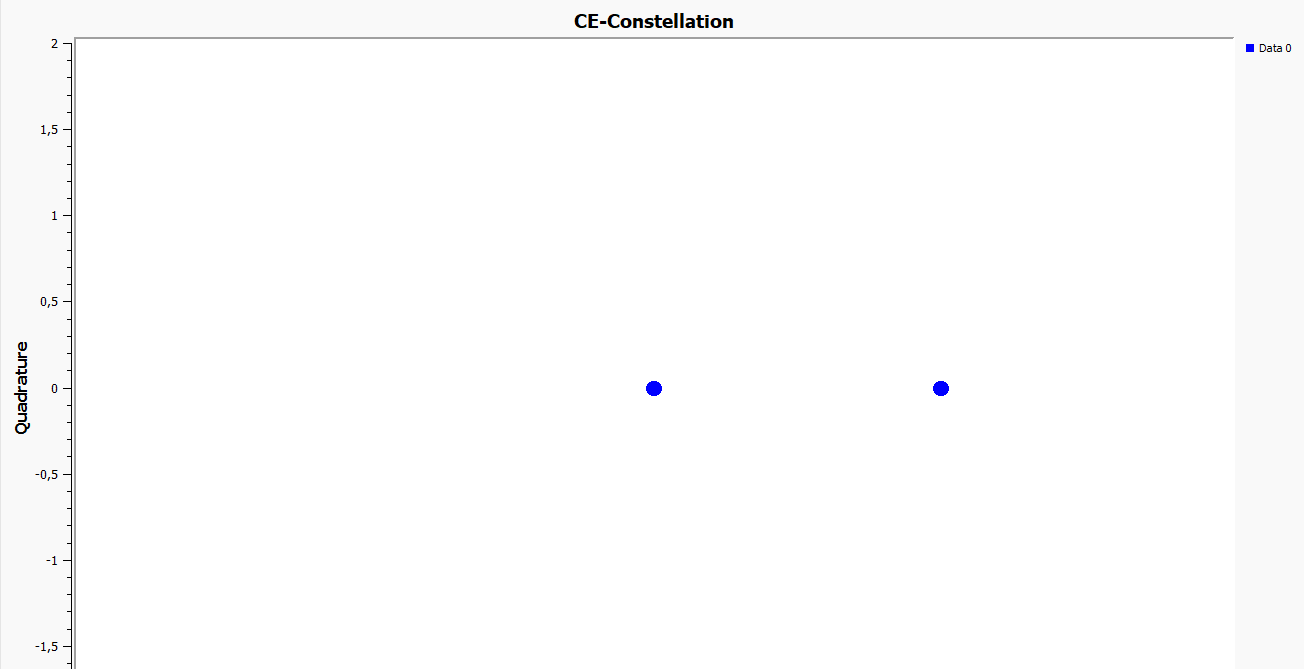
\includegraphics[width=0.9\columnwidth]{images/ook-fc-0-32-250-k.png}
    \caption{OOK Fc= 0/32/250 k}
    \label{fig:ook_fc_0_32_250_k}
\end{figure}

\subsection{B. Modulación Binary Phase-Shift Keying (BPSK)}

La modulación BPSK es una técnica de modulación digital en la que la información 
binaria se transmite modificando la \textbf{fase} de una señal portadora. En este 
caso, cada bit se representa mediante una de dos posibles fases, separadas por 180°.

\begin{figure}[H]
    \centering
    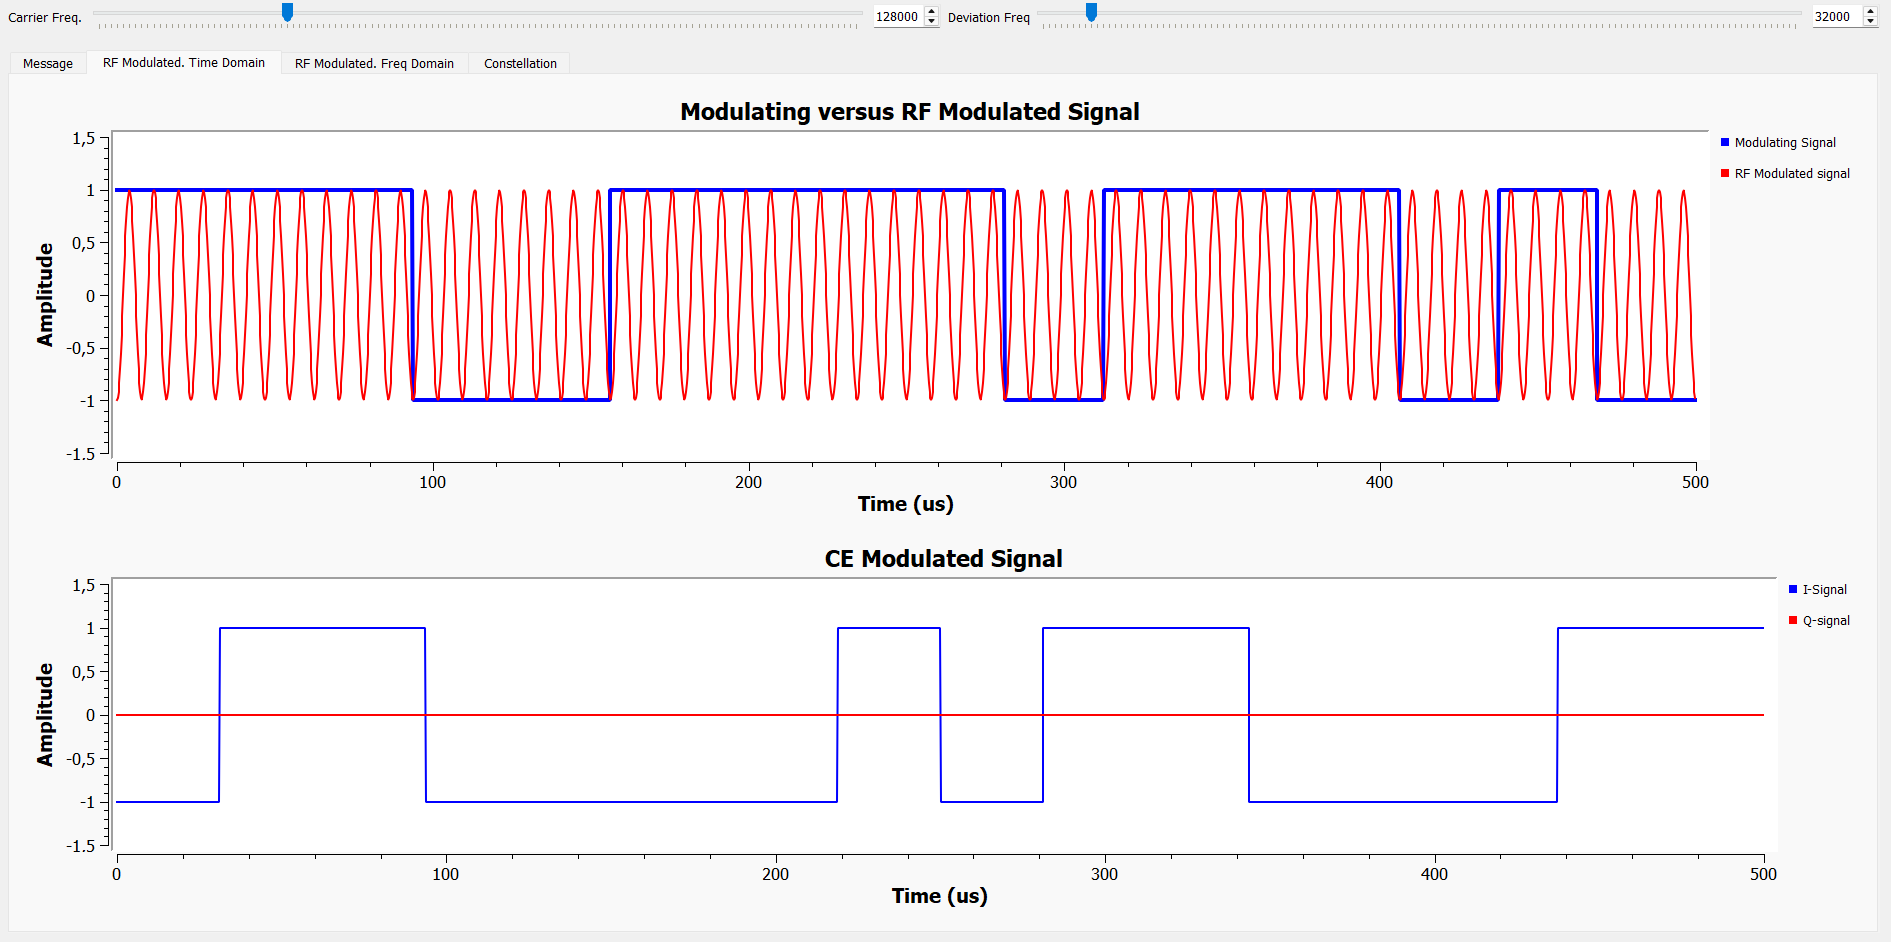
\includegraphics[width=0.9\columnwidth]{images/Rf_modulated_time_bpsk.png}
    \caption{BPSK Fc= 128k}
    \label{fig:bpsk_time}
\end{figure}

En esta modulación:
\begin{itemize}
    \item El bit \textbf{1} se transmite con una fase de 0°.
    \item El bit \textbf{0} se transmite con una fase de 180°.
\end{itemize}

Matemáticamente, la señal puede expresarse como:

\begin{equation}
    s(t) = A\cos(2\pi f_c t + \pi b(t)),
\end{equation}

donde $A$ es la amplitud, $f_c$ la frecuencia de la portadora y $b(t)$ representa 
el bit transmitido (0 o 1).

En la versión EC (envolvente compleja), la señal BPSK se representa únicamente 
por su componente en fase (I-Signal), la cual alterna entre $+1$ y $-1$, mientras 
que la componente en cuadratura (Q-Signal) permanece en cero, confirmando que 
toda la información se transmite mediante cambios de fase.

La principal ventaja de BPSK es su \textbf{alta inmunidad al ruido} en comparación 
con otras modulaciones de amplitud. Debido a que solo se utilizan dos fases bien 
definidas, la detección de los bits es más robusta ante interferencias y 
distorsiones del canal.

Sin embargo, transmite un solo bit por símbolo, por lo que su eficiencia 
espectral es menor que en modulaciones con más niveles de fase, como QPSK o 8-PSK.

\begin{figure}[H]
    \centering
    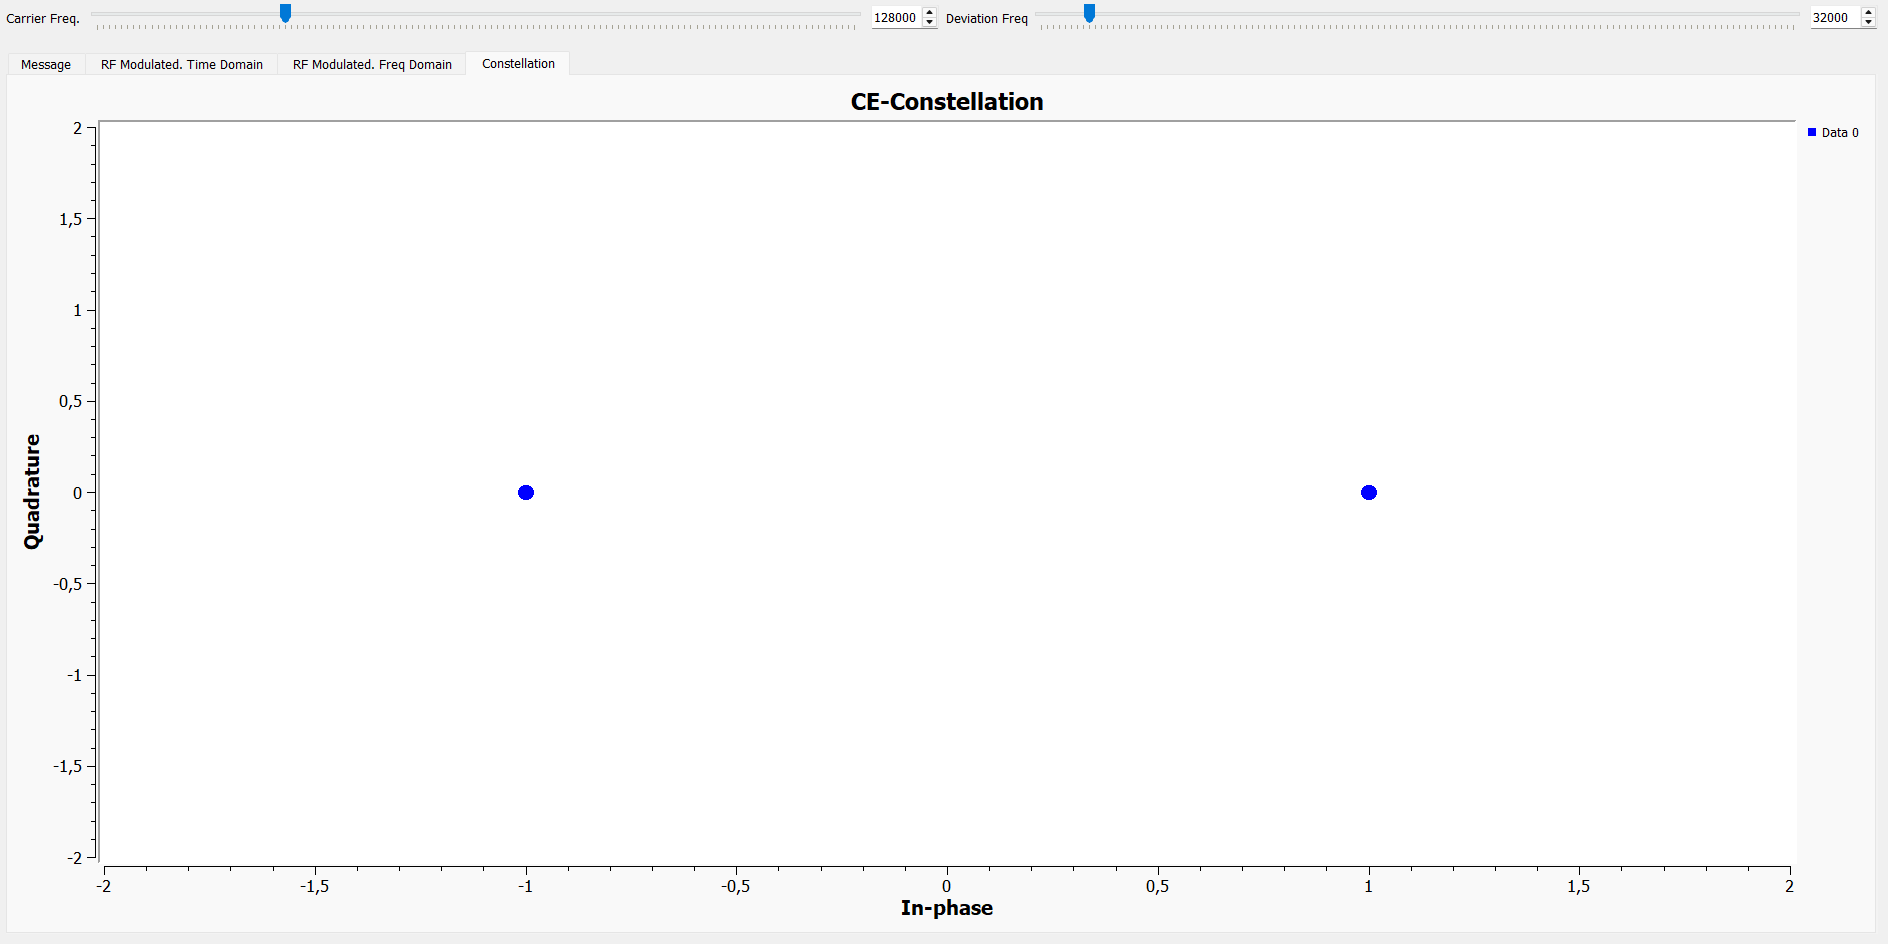
\includegraphics[width=0.9\columnwidth]{images/Constellation_bpsk.png}
    \caption{BPSK constelación Fc= 128k}
    \label{fig:bpsk_constelacion}
\end{figure}

La modulación BPSK presenta las siguientes características en el dominio 
de la frecuencia:

\begin{figure}[H]
    \centering
    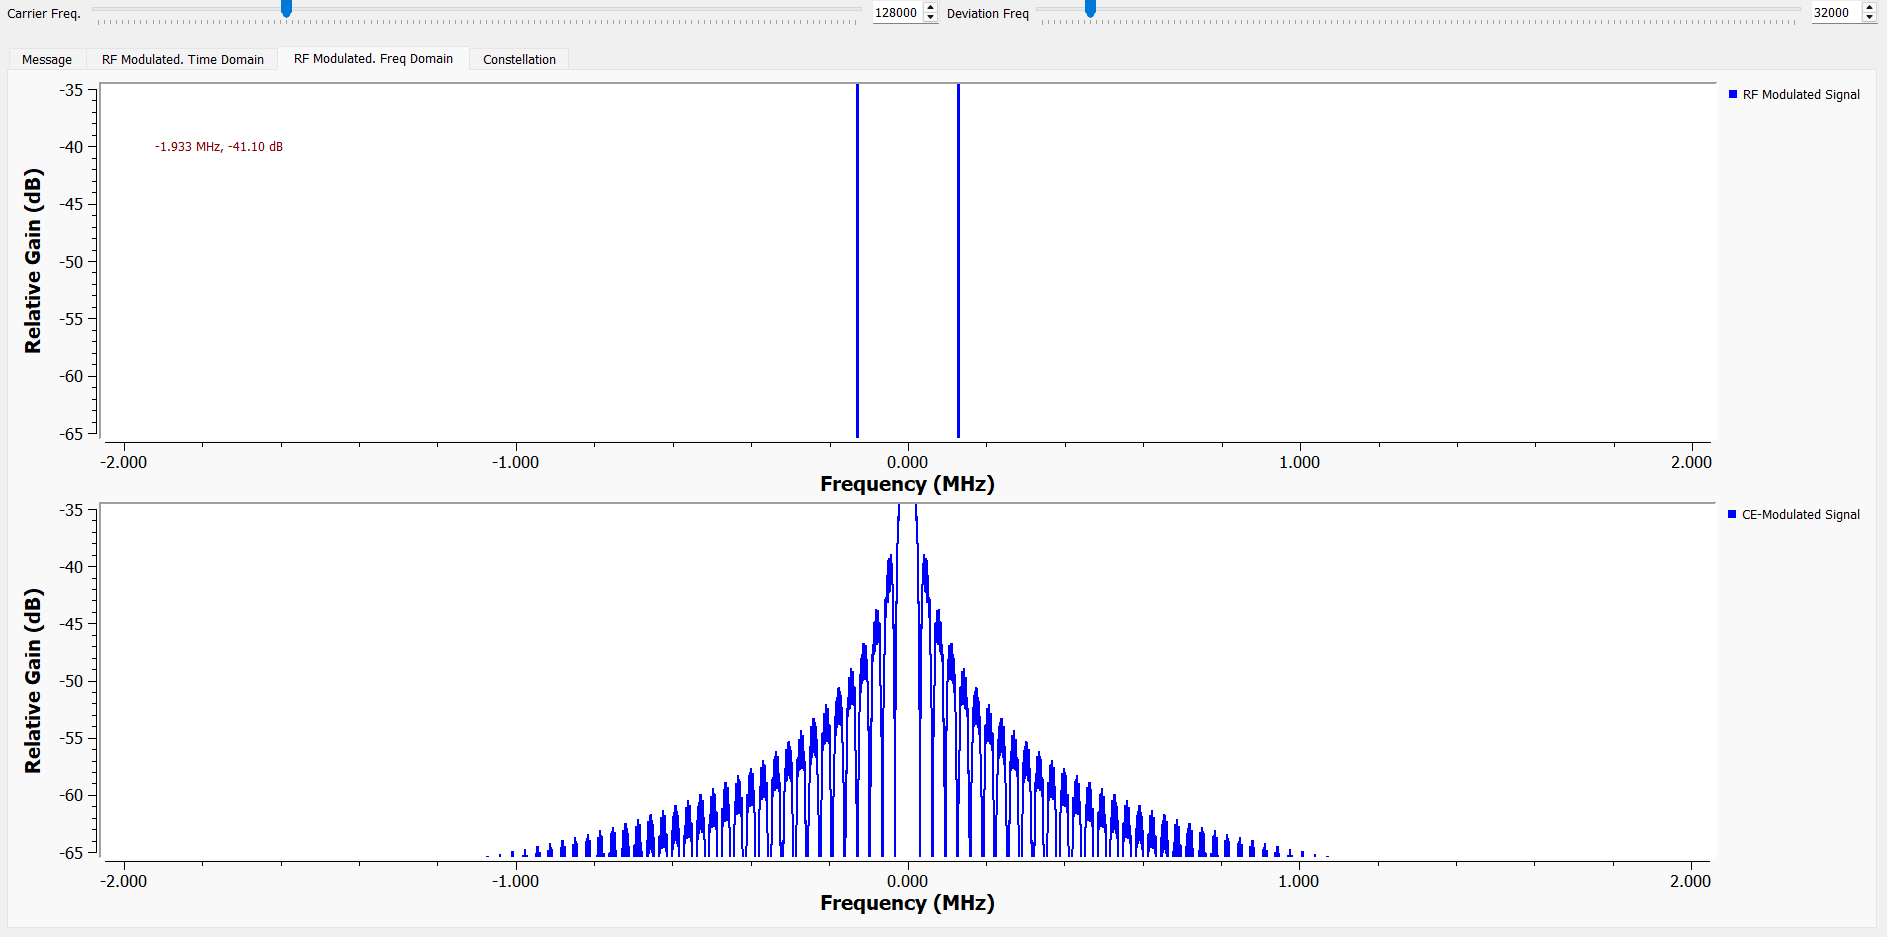
\includegraphics[width=0.9\columnwidth]{images/Rf_modulated_freq_bpsk.png}
    \caption{BPSK RF Modulated/Freq Domain fc= 128k}
    \label{fig:bpsk_freq}
\end{figure}

Adicionalmente en frecuencia para esta modulación se tiene:
\begin{itemize}
    \item \textbf{Centro espectral}: 128 kHz (frecuencia de portadora)
    \item \textbf{Simetría perfecta}: Lóbulos idénticos alrededor de $f_c$
    \item \textbf{Forma sinc$^2$}: Resultado de los pulsos rectangulares BPSK
\end{itemize}

La modulación BPSK es ampliamente utilizada en sistemas satelitales, enlaces 
de microondas, comunicaciones inalámbricas y sistemas de navegación, donde 
la fiabilidad de la transmisión es prioritaria sobre la velocidad de datos.

\subsection*{Variación de $f_c$ y $f_d$}

Al variar $f_c$ de 64k a 256k se observa que la señal RF cambia su densidad 
de ciclos por símbolo, mientras que la señal EC permanece inalterada, 
demostrando que la versión EC es independiente de $f_c$.

\begin{figure}[H]
    \centering
    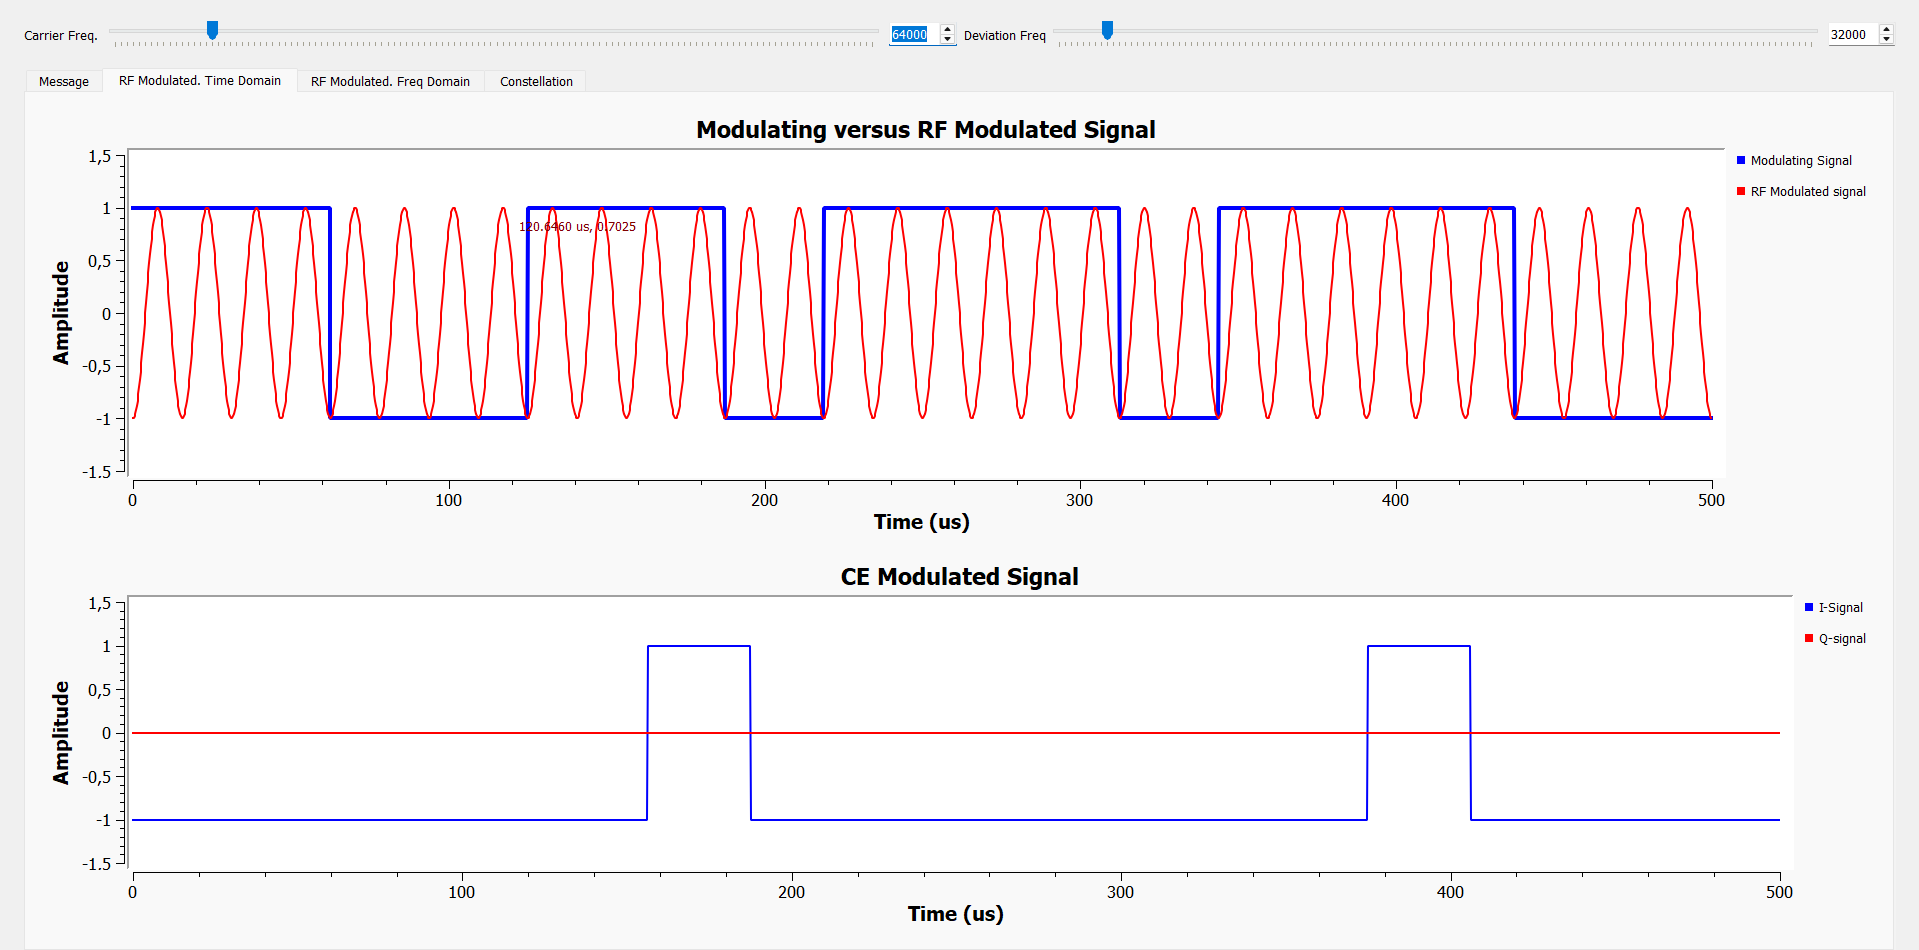
\includegraphics[width=0.9\columnwidth]{images/FC1.png}
    \caption{BPSK fc= 64k, fd= 32k}
    \label{fig:bpsk_fc64}
\end{figure}

\begin{figure}[H]
    \centering
    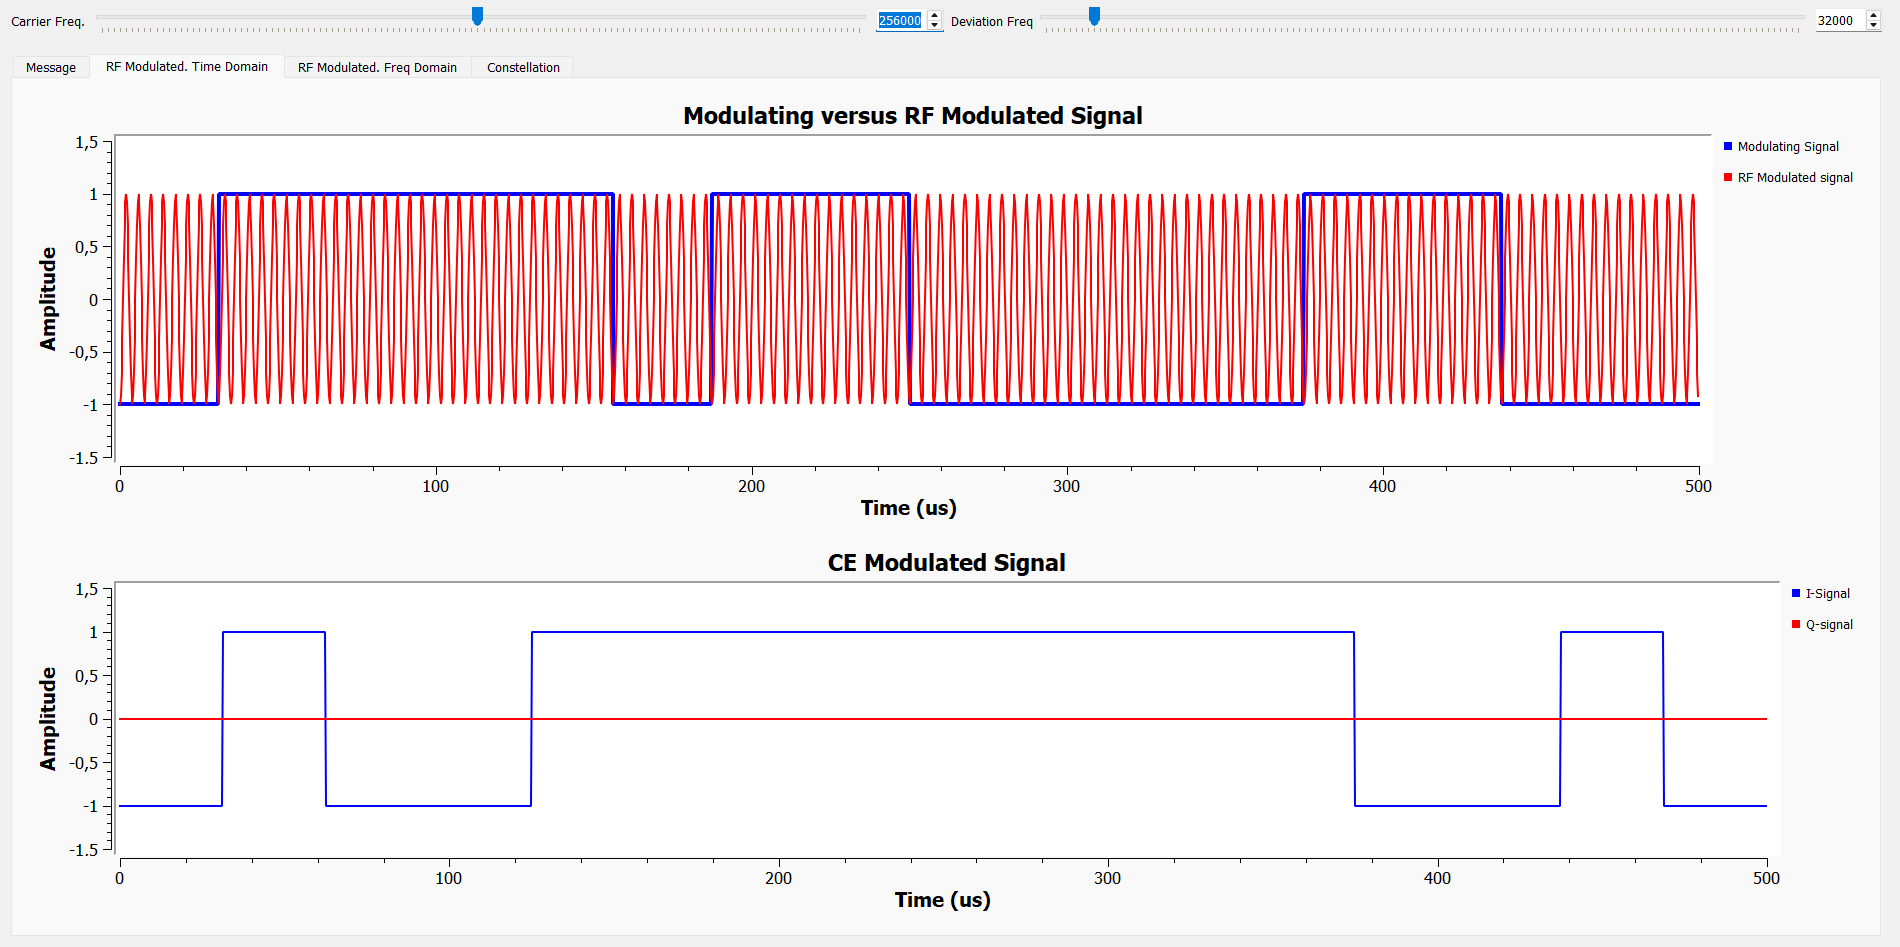
\includegraphics[width=0.9\columnwidth]{images/FC2.png}
    \caption{BPSK fc= 256k, fd= 32k}
    \label{fig:bpsk_fc256}
\end{figure}

Al aumentar $f_d$ a 64k las transiciones entre símbolos ocurren más 
rápido, aumentando el ancho de banda ocupado.

\begin{figure}[H]
    \centering
    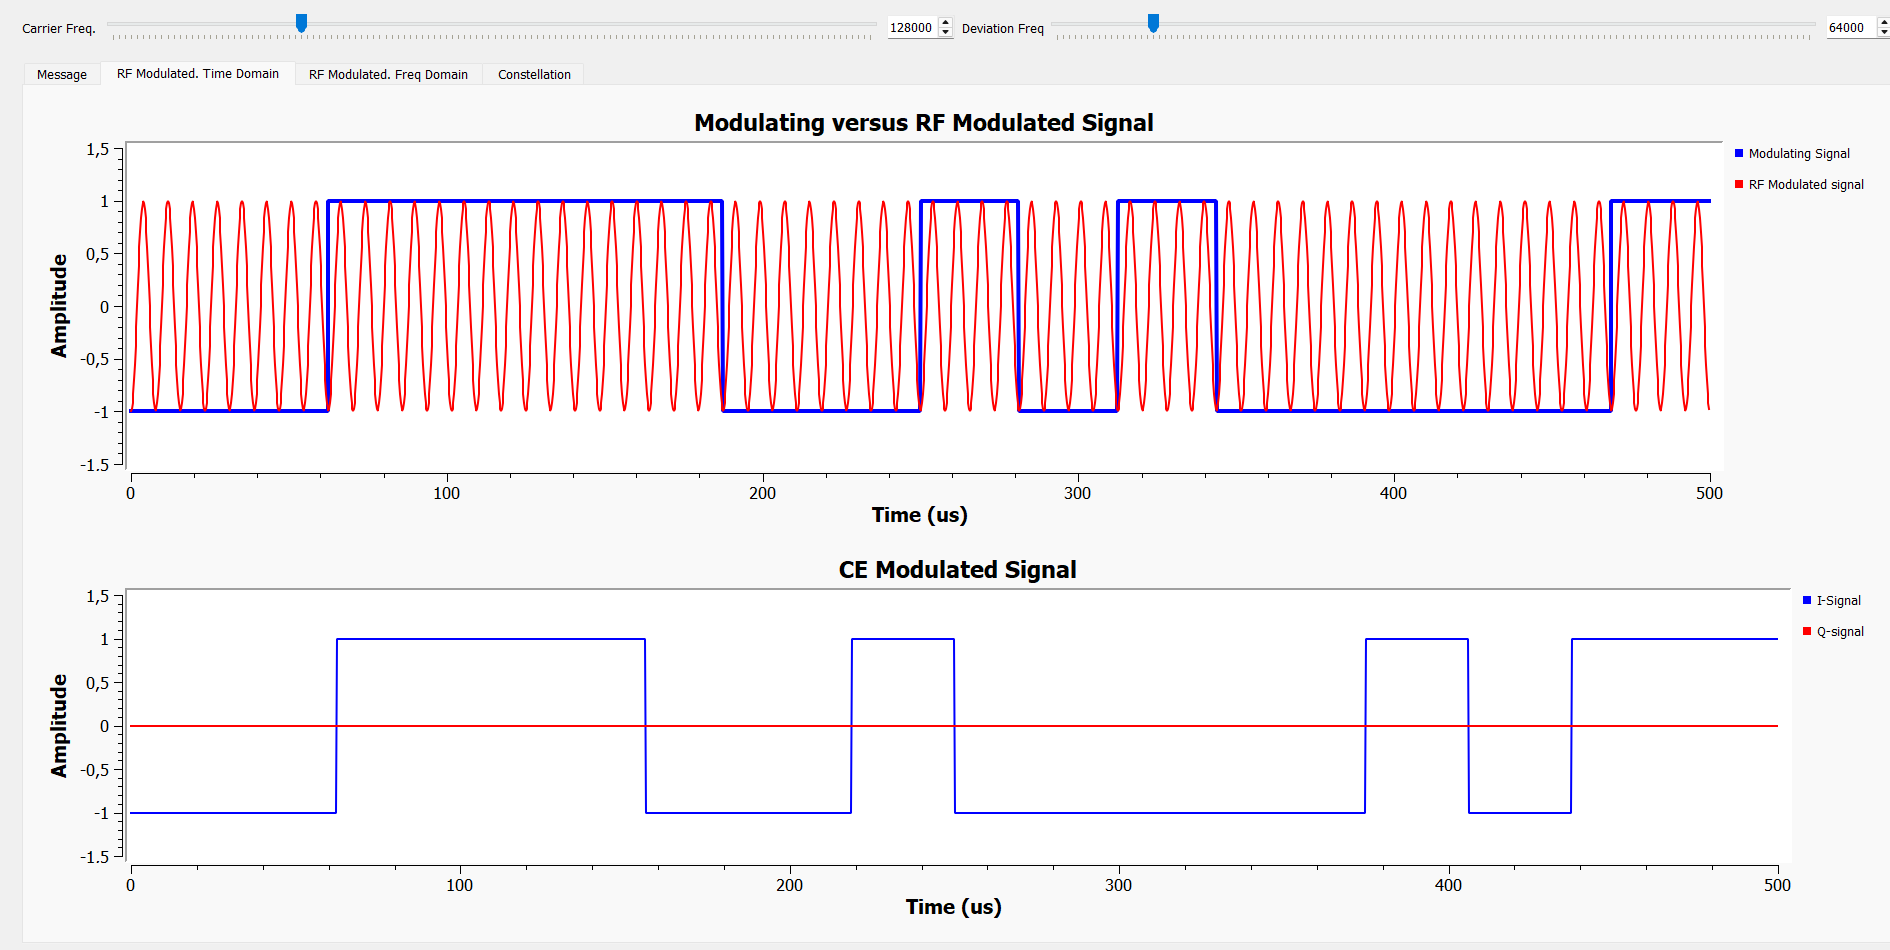
\includegraphics[width=0.9\columnwidth]{images/FC3.png}
    \caption{BPSK fc= 128k, fd= 64k}
    \label{fig:bpsk_fd64}
\end{figure}



\subsection{Resultados en el dominio del tiempo}

La Fig.~\ref{fig:tiempo_fsk} muestra la señal modulante bipolar superpuesta con 
la señal RF modulada en FSK. Se observan claramente dos frecuencias instantáneas 
distintas: $f_c - f_d$ para el bit ``0'' y $f_c + f_d$ para el bit ``1''.


\begin{figure}[H]
    \centering
    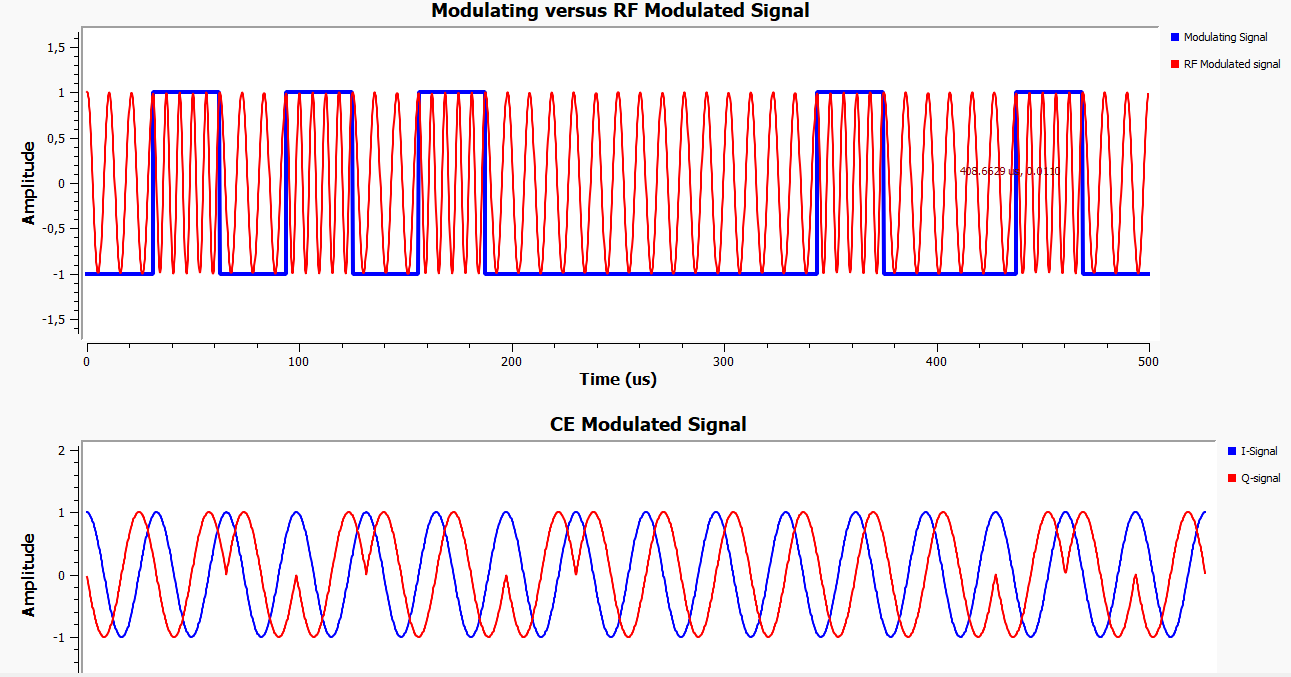
\includegraphics[width=0.48\textwidth]{images/tiempo_fsk.png}
    \caption{Dominio del tiempo: señal modulante bipolar (azul) y señal FSK en RF 
             (rojo) con $f_c=128\,\text{kHz}$, $f_d=32\,\text{kHz}$. Los segmentos 
             de bit ``0'' y ``1'' presentan frecuencias instantáneas $f_c \mp f_d$.}
    \label{fig:tiempo_fsk}
\end{figure}

Al variar $f_c$ con $f_d$ fijo, la densidad de ciclos por símbolo cambia en la 
señal RF pero la EC permanece invariante, lo que confirma que 
$s_{CE}[n] = e^{j\theta[n]}$ no depende de la portadora. Al variar $f_d$ con $f_c$ 
fijo, la diferencia entre las dos frecuencias instantáneas se hace más o menos 
evidente tanto en RF como en la velocidad de rotación del fasor CE.

\subsection{Resultados en el dominio de la frecuencia}

La Fig.~\ref{fig:espectro_fsk} presenta los espectros RF y CE de la señal FSK.


\begin{figure}[H]
    \centering
    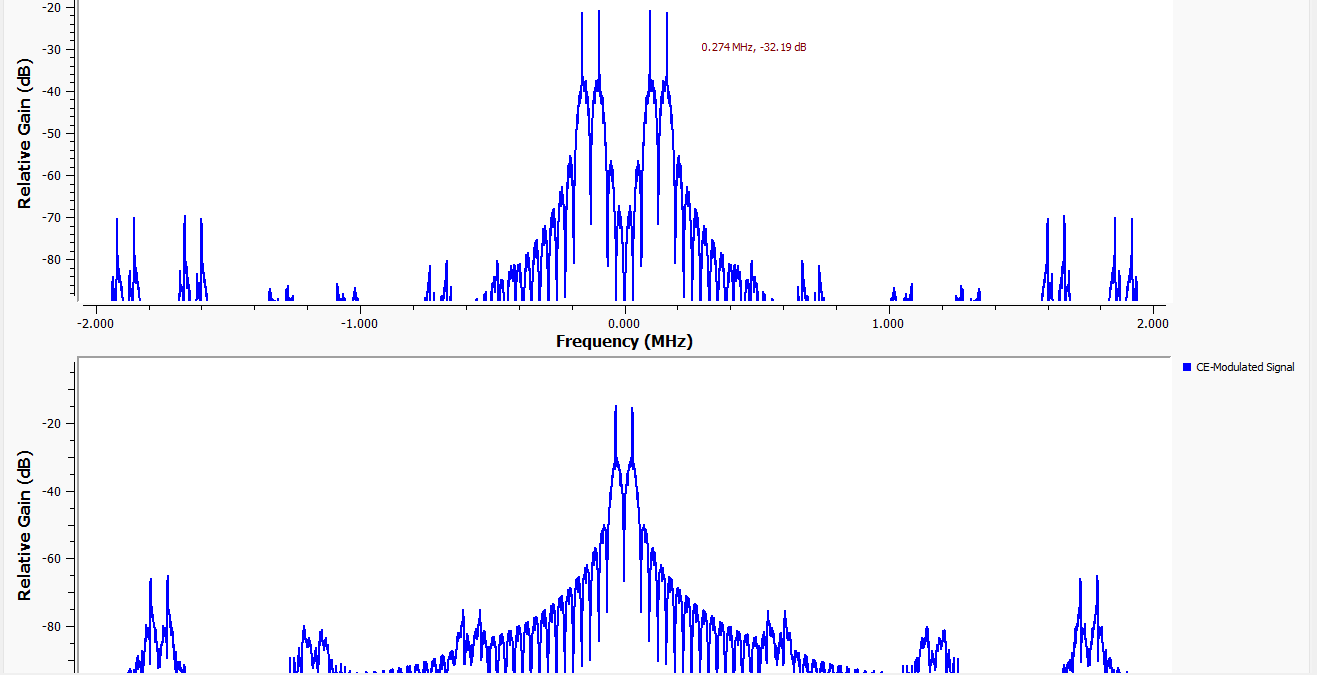
\includegraphics[width=0.48\textwidth]{images/espectro_fsk.png}
    \caption{Espectro de potencia de la señal FSK. \textbf{(a)} Versión RF: picos 
             en $f_c \pm f_d = \{96, 160\}\,\text{kHz}$. \textbf{(b)} Versión CE: 
             picos en $\pm f_d = \pm 32\,\text{kHz}$, independiente de $f_c$.}
    \label{fig:espectro_fsk}
\end{figure}

Para minimizar el solapamiento espectral, la separación entre lóbulos $2f_d$ debe 
superar el ancho del lóbulo principal $\approx 2R_b$, imponiendo la condición de 
ortogonalidad mínima $f_d \geq R_b/2 = 16\,\text{kHz}$. La 
Fig.~\ref{fig:espectro_comp} compara dos configuraciones: $f_d = 8\,\text{kHz}$ 
(solapamiento) y $f_d = 48\,\text{kHz}$ (separación óptima).


\begin{figure}[H]
    \centering
    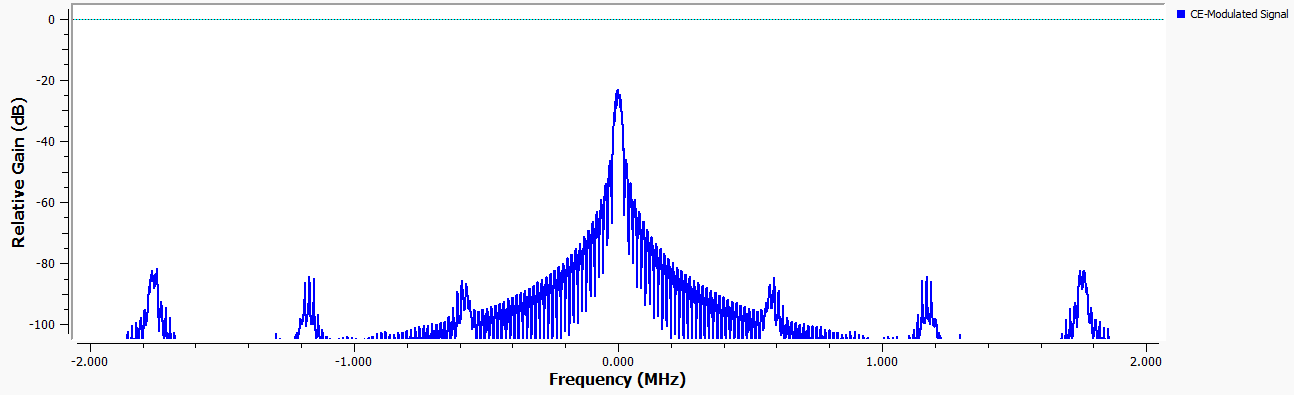
\includegraphics[width=0.23\textwidth]{images/espectro_fd8.png}\hfill
    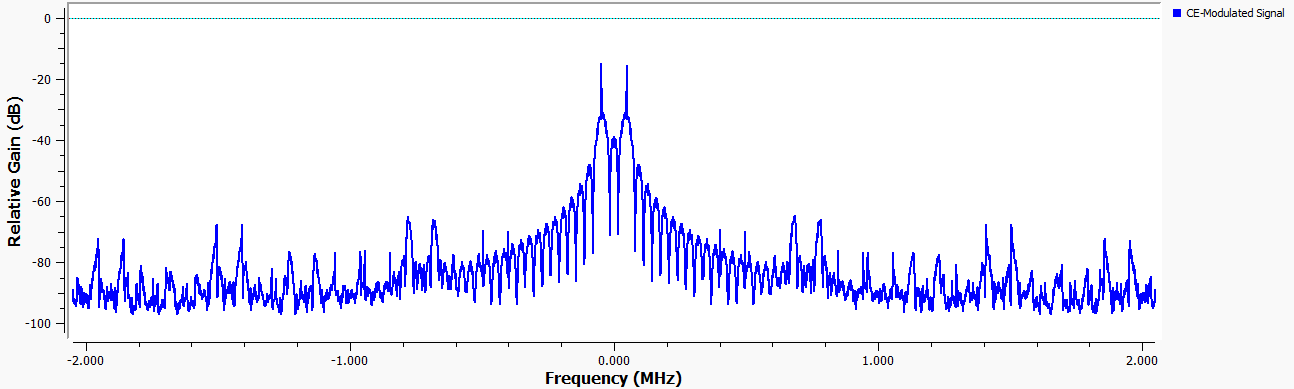
\includegraphics[width=0.23\textwidth]{images/espectro_fd48.png}
    \caption{Espectro CE comparativo. \textbf{Izq.:} $f_d=8\,\text{kHz}$, 
             solapamiento entre lóbulos. \textbf{Der.:} $f_d=48\,\text{kHz}$, 
             separación óptima con mínimo ancho de banda total.}
    \label{fig:espectro_comp}
\end{figure}

\subsection{Constelación IQ de la señal FSK}
\label{subsec:constelacion}

La Fig.~\ref{fig:constelacion_fsk} muestra la constelación IQ de la señal FSK en 
versión CE para dos valores de $f_d$.


\begin{figure}[H]
    \centering
    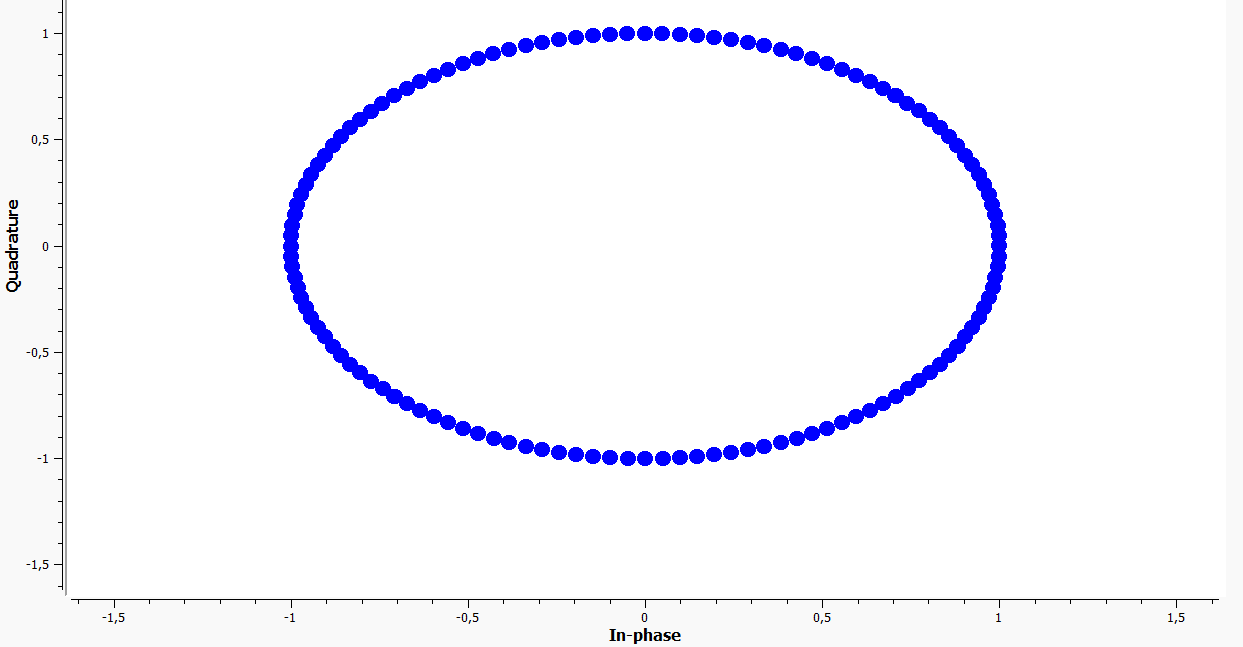
\includegraphics[width=0.23\textwidth]{images/const_fd32.png}\hfill
    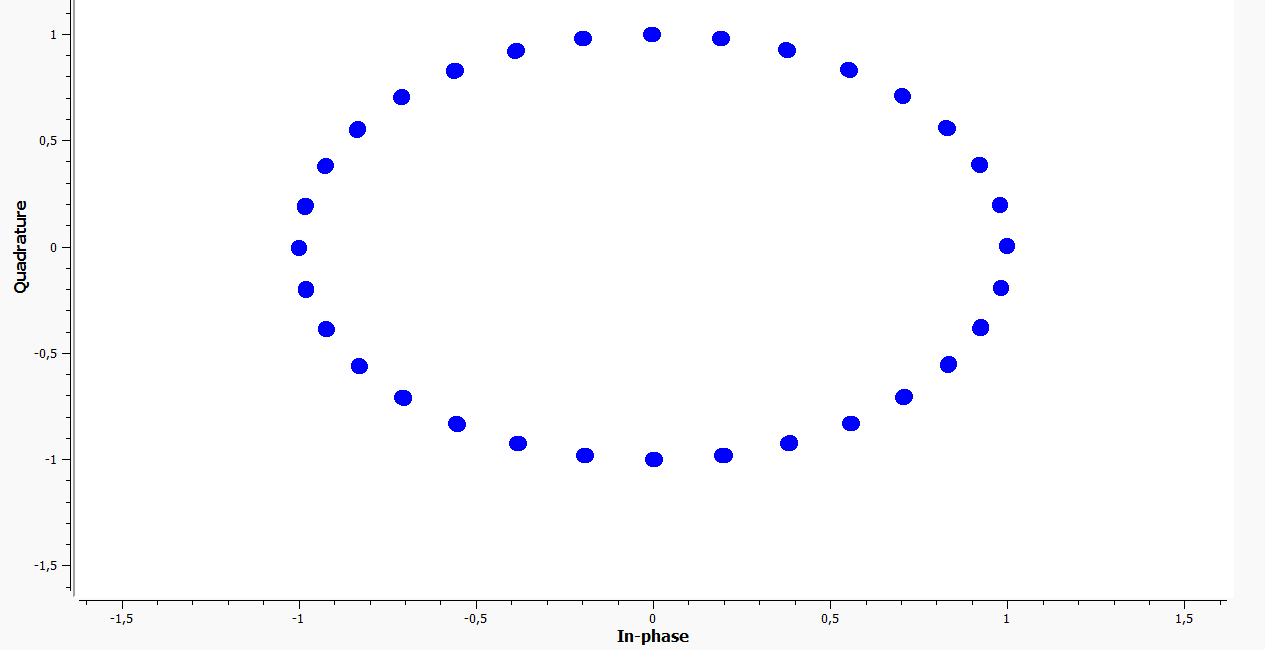
\includegraphics[width=0.23\textwidth]{images/const_fd128.png}
    \caption{Constelación IQ de FSK. \textbf{Izq.:} $f_d=32\,\text{kHz}$, arco 
             sobre la circunferencia unitaria. \textbf{Der.:} $f_d=128\,\text{kHz}$, 
             círculo completo. En ambos casos el módulo $|s_{CE}|=1$.}
    \label{fig:constelacion_fsk}
\end{figure}

Dado que $s_{CE}[n] = e^{j\theta[n]}$ tiene módulo unitario para todo $n$, la 
constelación de FSK siempre describe una trayectoria sobre la circunferencia de 
radio 1. Esto contrasta con BPSK (dos puntos en $\pm 1$) y OOK (dos puntos en 
$0$ y $+1$), y refleja la propiedad de envolvente constante de FSK, que la hace 
robusta frente a amplificadores no lineales[2].


\section{Conclusiones}
Se determinó la relación entre las señales de Radiofrecuencia (RF) y su representación en Envolvente Compleja (EC), lo cual permitió evidenciar que dicha conversión optimiza el procesamiento digital. Al operar directamente en banda base, se logra reducir la carga computacional sin comprometer la integridad de la información relevante.

La modulación BPSK codifica información mediante cambios de fase de 180°, 
otorgándole alta inmunidad al ruido frente a modulaciones de amplitud. 
La versión RF opera en paso banda sobre la portadora, mientras que la 
versión EC revela la esencia matemática de la modulación: toda la 
información reside en la componente I, con Q nula, confirmando que BPSK 
es una modulación unidimensional, base de sistemas modernos como 
LTE y 5G.
\section{Referencias}
[1] B. P. Lathi, Modern Digital and Analog Communication Systems, 4ta ed. Oxford University Press, 2009.
[2] S. Haykin, Communication Systems, 4ta ed. Wiley, 2001
\end{document}
